\documentclass[12pt, letterpaper]{article}

\usepackage{amsmath}
\usepackage{booktabs}
\usepackage{graphicx}
\usepackage{hyperref}
\usepackage{microtype}

\title{Machine Learning Engineer Nanodegree\\Capstone Report}
\author{Daniel Chao Zhou}
\date{31 December 2019}

\begin{document}

\maketitle

\section{Definition} % (approx. 1-2 pages)

\subsection{Project Overview}

\paragraph{}
The stock market prediction has been identified as a significant practical problem in the economic field. Trading algorithms rather than humans performed over 80\% of trading in the stock market and the FOREX market. In the crypto-currency market, algorithmic trading is also a hot topic among investors. However, timely and accurate prediction of the market is generally regarded as one of the most challenging problems, since the environment is profoundly affected by volatile political-economic factors, such as legislative acts, political unrest, and mass irrational panic.

\paragraph{}
There are many studies regarding algorithmic trading in financial markets based on machine learning, where recurrent neural network (RNN) and reinforcement learning (RL) are being popular in recent years. In this study, a Bitcoin price predictor based on long short-term memory (LSTM, a variant of RNN) is presented.

\subsection{Problem Statement}

\paragraph{}
Given the trading data of a Bitcoin futures contract with each time step indicating one minute, the goal is to build a predictor for the volume-weighted average price (VWAP) of the next minute.

\paragraph{}
Two predictors, an LSTM model as solution and a linear model as benchmark will be built and compared with the metrics as discussed as follows.

\subsection{Metrics}

\paragraph{}
The mean squared error (MSE) between labels \(y\) and predictions \(\hat y\) will be used to evaluate the performance of both of the benchmark model and the solution model. For a given integer \(N\) and a time-series dataset, all consecutive sub-sequence of the time-series with length \(N\) will be used and equally contribute to the final MSE\@.

\section{Analysis} % (approx. 2-4 pages)

\subsection{Data Exploration}

\paragraph{}
In this study, trading data of BitMEX's XBTZ19 contract, which is a Bitcoin futures contract expiring in December 2019, will be used to train and test the predictor. The dataset could be fetched from BitMEX's official API without charge of fee. The API concerned with the desired data is documented at \url{https://www.bitmex.com/api/explorer/#!/Trade/Trade_getBucketed}.

\paragraph{}
The dataset is a table that each row indicates one minute and each column indicates a specific data described as Table~\ref{table:column-header}. Note that \texttt{open} is not defined as the price of the first trade in the specific time step, which in an unconventional definition and does not apply to other data sources.

\begin{table}
    \caption{column header semantics}%
    \label{table:column-header}
    \centering
    \begin{tabular}{ll}
        \toprule
        \texttt{high,low} & highest/lowest price (two columns) \\
        \texttt{close} & price of the last trade \\
        \texttt{open} & \texttt{close} of the last time step \\
        \texttt{vwap} & volume-weighted average price (VWAP) \\
        \texttt{foreignNotional} & traded amount in units of US dollar \\
        \texttt{homeNotional} & traded amount in units of Bitcoin \\
        \texttt{trades} & number of trades \\
        \texttt{volume} & alias of \texttt{foreignNotional} \\
        \bottomrule
    \end{tabular}
\end{table}

\paragraph{}
The dataset is formulated as \(\{x_t|t=1,2,\dots,T\}\), where \(x_t\) is a vector of the data in minute \(t\), such that \(x_t=(\mathtt{open}_t,\mathtt{high}_t,\mathtt{low}_t,\mathtt{close}_t,\mathtt{vwap}_t,\dots)\). A small sample and basic statistics are given in Table~\ref{table:sample} and Table~\ref{table:statistics}.

\begin{table}
    \caption{head and tail part of the dataset}%
    \label{table:sample}
    \resizebox{\textwidth}{!}{
    \begin{tabular}{l|*8r}
        \toprule
        & open & high & low & close & vwap & foreignNotional & homeNotional & trades \\
        \midrule
        2019-06-14 08:31 & NaN & NaN & NaN & NaN & NaN & 0 & 0.000000 & 0 \\
        2019-06-14 08:32 & NaN & NaN & NaN & NaN & NaN & 0 & 0.000000 & 0 \\
        2019-06-14 08:33 & 8500.00 & 8500.00 & 8260.00 & 8260.00 & 8262.4143 & 201 & 0.024328 & 3 \\
        2019-06-14 08:34 & 8260.00 & 8390.00 & 8308.00 & 8308.00 & 8325.0083 & 13110 & 1.574852 & 7 \\
        2019-06-14 08:35 & 8308.00 & 8390.00 & 8319.50 & 8336.50 & 8322.9297 & 13200 & 1.585986 & 5 \\
        2019-06-14 08:36 & 8336.50 & 8317.50 & 8317.50 & 8317.50 & 8317.5000 & 10200 & 1.226346 & 3 \\
        2019-06-14 08:37 & 8317.50 & 8327.50 & 8327.50 & 8327.50 & 8328.0000 & 500 & 0.060040 & 1 \\
        2019-06-14 08:38 & 8327.50 & 8366.50 & 8362.50 & 8362.50 & 8365.4007 & 4001 & 0.478290 & 5 \\
        \dots & \dots & \dots & \dots & \dots & \dots & \dots & \dots & \dots \\
        2019-12-27 11:54 & 7151.00 & 7155.50 & 7135.00 & 7137.50 & 7149.4960 & 632224 & 88.434680 & 62 \\
        2019-12-27 11:55 & 7137.50 & 7149.50 & 7137.50 & 7149.00 & 7141.3269 & 60153 & 8.423772 & 44 \\
        2019-12-27 11:56 & 7149.00 & 7142.00 & 7140.50 & 7141.50 & 7140.8169 & 407108 & 57.015170 & 34 \\
        2019-12-27 11:57 & 7141.50 & 7149.50 & 7141.00 & 7141.50 & 7141.3269 & 325738 & 45.615289 & 22 \\
        2019-12-27 11:58 & 7141.50 & 7150.00 & 7141.50 & 7150.00 & 7149.4960 & 390967 & 54.686307 & 31 \\
        2019-12-27 11:59 & 7150.00 & 7150.00 & 7141.00 & 7148.50 & 7142.8571 & 540701 & 75.700246 & 30 \\
        2019-12-27 12:00 & 7148.50 & 7148.50 & 7138.24 & 7138.24 & 7138.7778 & 41934166 & 5874.536073 & 59 \\
        2019-12-27 12:01 & 7138.24 & 7138.24 & 7138.24 & 7138.24 & NaN & 0 & 0.000000 & 0 \\
        \bottomrule
    \end{tabular}}
\end{table}

\begin{table}
    \caption{basic statistics of the dataset}%
    \label{table:statistics}
    \resizebox{\textwidth}{!}{
    \begin{tabular}{l|*8r}
        \toprule
        & open & high & low & close & vwap & foreignNotional & homeNotional & trades \\
        \midrule
        count & 282449.00 & 282449.00 & 282449.00 & 282449.00 & 243964.00 & 2.82e+05 & 282451.00 & 282451.00 \\
        mean & 9499.88 & 9502.96 & 9496.68 & 9499.87 & 9558.33 & 3.69e+04 & 3.94 & 23.43 \\
        std & 1621.16 & 1622.74 & 1619.51 & 1621.17 & 1632.99 & 1.37e+05 & 16.63 & 46.27 \\
        min & 6438.00 & 6443.50 & 6431.00 & 6438.00 & 6432.52 & 0.00e+00 & 0.00 & 0.00 \\
        25\% & 8158.00 & 8159.50 & 8157.00 & 8158.00 & 8180.62 & 6.05e+02 & 0.06 & 2.00 \\
        50\% & 9542.50 & 9546.00 & 9540.00 & 9542.50 & 9589.56 & 7.33e+03 & 0.77 & 10.00 \\
        75\% & 10616.50 & 10619.50 & 10614.00 & 10616.50 & 10656.43 & 3.20e+04 & 3.36 & 26.00 \\
        max & 14600.00 & 14600.00 & 14539.00 & 14600.00 & 14547.57 & 4.19e+07 & 5874.53 & 1529.00 \\
        \bottomrule
    \end{tabular}}
\end{table}

\subsection{Exploratory Visualization}

The VWAP and volume of the dataset is shown in Figure~\ref{fig:input}.

\begin{figure}
    \centering
    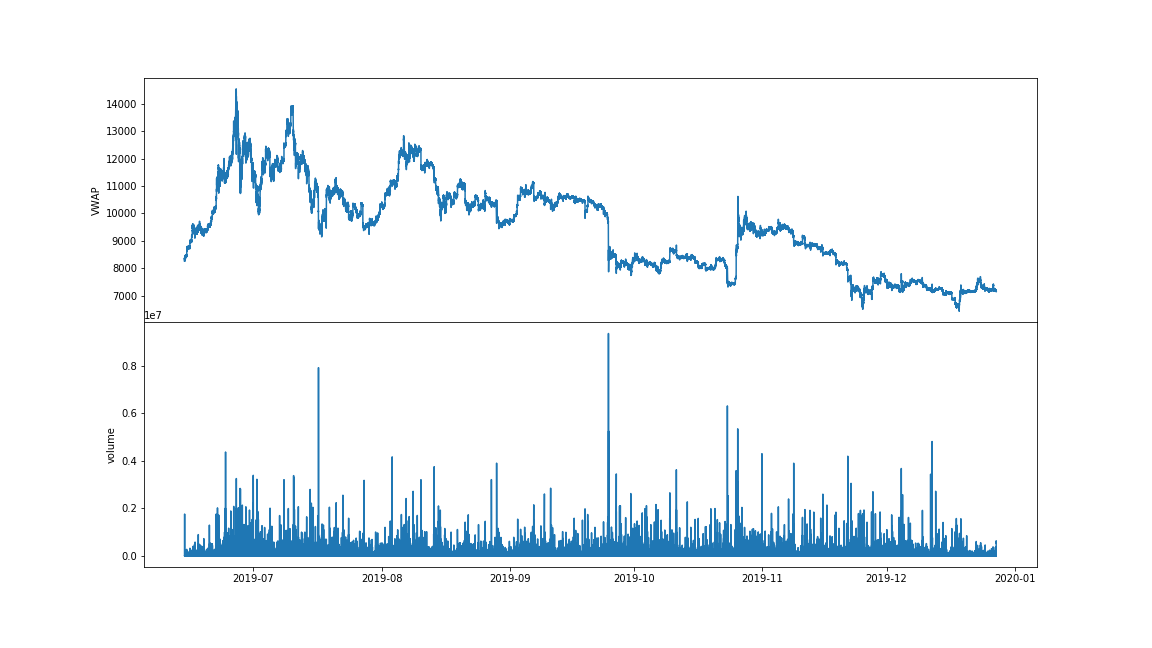
\includegraphics[width=\textwidth]{input.png}
    \caption{VWAP and volume of the dataset}%
    \label{fig:input}
\end{figure}

\subsection{Algorithms and Techniques}

\paragraph{}
The solution model consists of one LSTM layer and one linear layer. The LSTM layer is formally formulated as follows:

\begin{align*}
    i_t & =\sigma\left(W_{ii}x_t+b_{ii}+W_{hi}h_{(t-1)}+b_{hi}\right), \\
    f_t & =\sigma\left(W_{if}x_t+b_{if}+W_{hf}h_{(t-1)}+b_{hf}\right), \\
    g_t & =\tanh\left(W_{ig}x_t+b_{ig}+W_{hg}h_{(t-1)}+b_{hg}\right), \\
    o_t & =\sigma\left(W_{io}x_t+b_{io}+W_{ho}h_{(t-1)}+b_{ho}\right), \\
    c_t & =f_t*c_{(t-1)}+i_t*g_t, \\
    h_t & =o_t*\tanh(c_t).
\end{align*}

where \(h_t\) is the hidden state at time \(t\), \(c_t\) is the cell state at time \(t\), \(x_t\) is the input at time \(t\), and \(i_t\), \(f_t\), \(g_t\), \(o_t\) are the input, forget, cell, and output gates, respectively. \(\sigma\) is the sigmoid function, and \(*\) is the Hadamard product.

\subsection{Benchmark}

\paragraph{}
The benchmark model consists of two linear regression layers:

\begin{align*}
    h & =\mathrm{ReLU}\left(xA_1+b_1\right), \\
    y  & =hA_2+b_2.
\end{align*}

\section{Methodology} % (approx. 3-5 pages)

\subsection{Data Preprocessing}

\paragraph{}
Data preprocessing steps are listed as follows.

\paragraph{Crawling} Since new data are generating every minute, new rows could be fetched from the data source. The crawler should be able to handle locally cached data and progressively persisting new data.

\paragraph{Column dropping} Columns \texttt{open} and \texttt{volume} do not provide new information and are dropped.

\paragraph{Null filling} For time steps that do not contain any trades, the corresponding \texttt{vwap} columns are null. These items will be propagated with last valid observation with \texttt{pandas.DataFrame.ffill()}.

\paragraph{Feature engineering} Moving average convergence/divergence (MACD) with short period of 12 and long period of 26, and relative strength index (RSI) with dataframe of 14, are calculated and appended as extra features for the following training and evaluating.

\paragraph{Normalisation} All features will be normalised.

\paragraph{Labelling} Each row will be labelled a learning target, with the VWAP of the next row.

\paragraph{Splitting} The entire dataset will be split without shuffling into three consecutive parts for training, validation, and testing, while the lengths proportionate to 6:2:2.

\subsection{Implementation}

\paragraph{}
MSE and the LSTM model could be easily implemented with PyTorch's builtin \texttt{torch.nn.MSELoss} class and \texttt{torch.nn.LSTM} class.

\subsection{Refinement}

\paragraph{}
The learning rate is automatically adjusted with the scheduler \\\texttt{torch.optim.lr\_scheduler.StepLR}. Moreover, the number of dimensions of the hidden layer are tuned with AWS SageMaker's hyperparameter tuning, which suggests that

\end{document}

In this section, you will need to discuss the process of improvement you made upon the algorithms and techniques you used in your implementation. For example, adjusting parameters for certain models to acquire improved solutions would fall under the refinement category. Your initial and final solutions should be reported, as well as any significant intermediate results as necessary. Questions to ask yourself when writing this section:

- _Has an initial solution been found and clearly reported?_
- _Is the process of improvement clearly documented, such as what techniques were used?_
- _Are intermediate and final solutions clearly reported as the process is improved?_

\section{Results} % (approx. 2-3 pages)

\begin{figure}
    \centering
    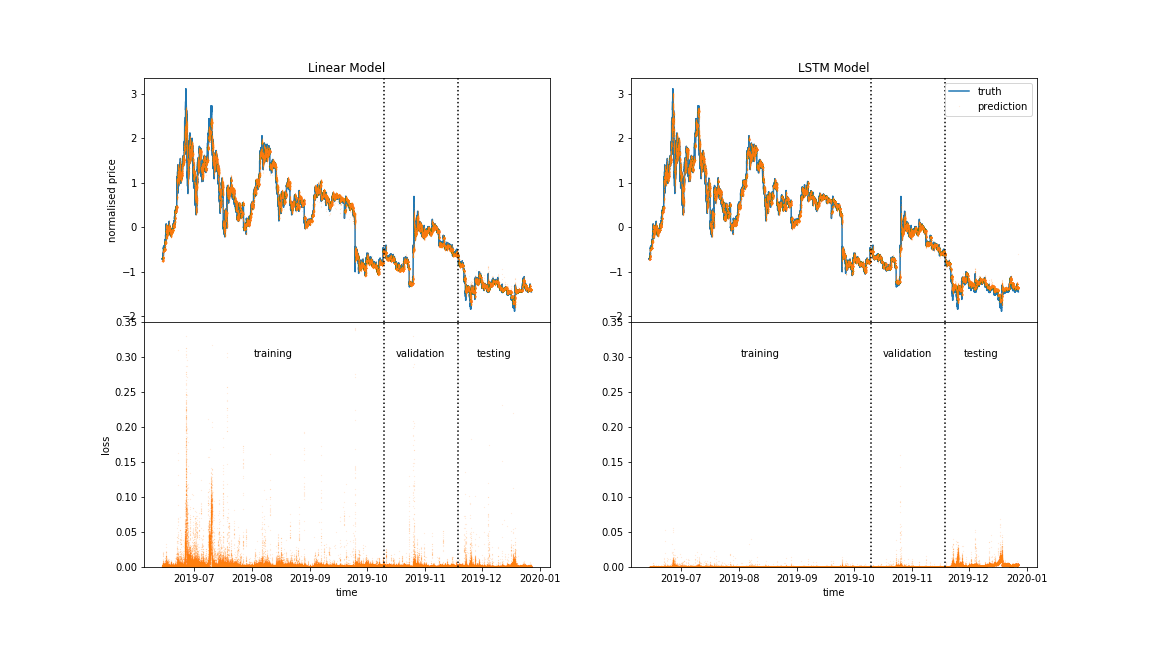
\includegraphics[width=\textwidth]{output.png}
    \caption{blah blah}%
    \label{fig:output}
\end{figure}

\subsection{Model Evaluation and Validation}

In this section, the final model and any supporting qualities should be evaluated in detail. It should be clear how the final model was derived and why this model was chosen. In addition, some type of analysis should be used to validate the robustness of this model and its solution, such as manipulating the input data or environment to see how the model’s solution is affected (this is called sensitivity analysis). Questions to ask yourself when writing this section:

- _Is the final model reasonable and aligning with solution expectations? Are the final parameters of the model appropriate?_
- _Has the final model been tested with various inputs to evaluate whether the model generalizes well to unseen data?_
- _Is the model robust enough for the problem? Do small perturbations (changes) in training data or the input space greatly affect the results?_
- _Can results found from the model be trusted?_

\subsection{Justification}

In this section, your model’s final solution and its results should be compared to the benchmark you established earlier in the project using some type of statistical analysis. You should also justify whether these results and the solution are significant enough to have solved the problem posed in the project. Questions to ask yourself when writing this section:

- _Are the final results found stronger than the benchmark result reported earlier?_
- _Have you thoroughly analyzed and discussed the final solution?_
- _Is the final solution significant enough to have solved the problem?_

\section{Conclusion} % (approx. 1-2 pages)

\subsection{Free-Form Visualization}

In this section, you will need to provide some form of visualization that emphasizes an important quality about the project. It is much more free-form, but should reasonably support a significant result or characteristic about the problem that you want to discuss. Questions to ask yourself when writing this section:

- _Have you visualized a relevant or important quality about the problem, dataset, input data, or results?_
- _Is the visualization thoroughly analyzed and discussed?_
- _If a plot is provided, are the axes, title, and datum clearly defined?_

\subsection{Reflection}

In this section, you will summarize the entire end-to-end problem solution and discuss one or two particular aspects of the project you found interesting or difficult. You are expected to reflect on the project as a whole to show that you have a firm understanding of the entire process employed in your work. Questions to ask yourself when writing this section:

- _Have you thoroughly summarized the entire process you used for this project?_
- _Were there any interesting aspects of the project?_
- _Were there any difficult aspects of the project?_
- _Does the final model and solution fit your expectations for the problem, and should it be used in a general setting to solve these types of problems?_

\subsection{Improvement}

In this section, you will need to provide discussion as to how one aspect of the implementation you designed could be improved. As an example, consider ways your implementation can be made more general, and what would need to be modified. You do not need to make this improvement, but the potential solutions resulting from these changes are considered and compared/contrasted to your current solution. Questions to ask yourself when writing this section:

- _Are there further improvements that could be made on the algorithms or techniques you used in this project?_
- _Were there algorithms or techniques you researched that you did not know how to implement, but would consider using if you knew how?_
- _If you used your final solution as the new benchmark, do you think an even better solution exists?_

---

**Before submitting, ask yourself. . .**

- Does the project report you’ve written follow a well-organized structure similar to that of the project template?
- Is each section (particularly **Analysis** and **Methodology**) written in a clear, concise and specific fashion? Are there any ambiguous terms or phrases that need clarification?
- Would the intended audience of your project be able to understand your analysis, methods, and results?
- Have you properly proof-read your project report to assure there are minimal grammatical and spelling mistakes?
- Are all the resources used for this project correctly cited and referenced?
- Is the code that implements your solution easily readable and properly commented?
- Does the code execute without error and produce results similar to those reported?

[^bigiotti]: Bigiotti, Alessandro; Navarra, Alfredo (October 19, 2018), "Optimizing Automated Trading Systems", Advances in Intelligent Systems and Computing, Springer International Publishing, pp. 254–261, doi:10.1007/978-3-030-02351-5_30, ISBN 978-3-030-02350-8
